

\tikzset{every picture/.style={line width=0.75pt}} %set default line width to 0.75pt        

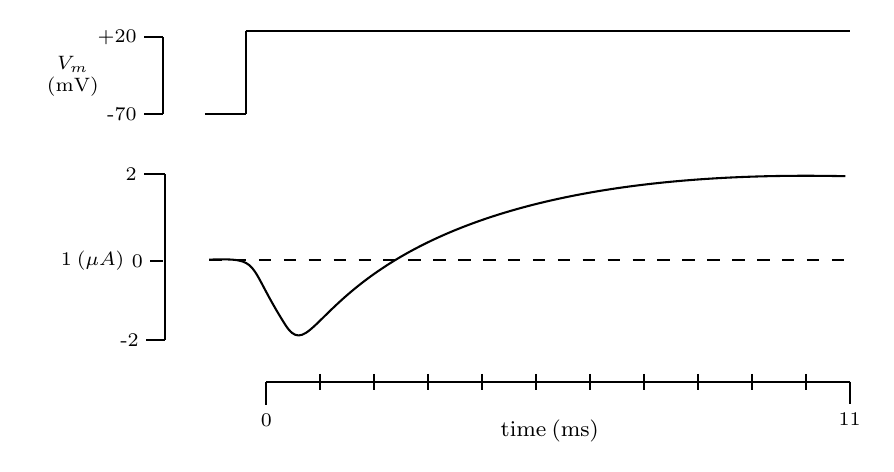
\begin{tikzpicture}[x=0.75pt,y=0.75pt,yscale=-1,xscale=1]
%uncomment if require: \path (0,263); %set diagram left start at 0, and has height of 263

%Straight Lines [id:da16011518847864004] 
\draw    (169.6,199) -- (450.6,199) (195.6,195) -- (195.6,203)(221.6,195) -- (221.6,203)(247.6,195) -- (247.6,203)(273.6,195) -- (273.6,203)(299.6,195) -- (299.6,203)(325.6,195) -- (325.6,203)(351.6,195) -- (351.6,203)(377.6,195) -- (377.6,203)(403.6,195) -- (403.6,203)(429.6,195) -- (429.6,203) ;
%Straight Lines [id:da6331484236419908] 
\draw    (169.6,199) -- (169.6,209.8) ;
%Straight Lines [id:da9468556493718451] 
\draw    (450.6,198.8) -- (450.6,209.6) ;
%Straight Lines [id:da24916388579329574] 
\draw  [dash pattern={on 4.5pt off 4.5pt}]  (142,140) -- (452.6,140) ;
%Straight Lines [id:da9306867894592372] 
\draw    (120.6,178.8) -- (120.6,98.8) ;
%Straight Lines [id:da5216250289907107] 
\draw    (120.6,98.8) -- (110.6,98.8) ;
%Straight Lines [id:da23662949375459186] 
\draw    (120.6,178.8) -- (111.6,178.8) ;
%Straight Lines [id:da29778043966934653] 
\draw    (119.6,140.8) -- (113.6,140.8) ;
%Straight Lines [id:da8763352921223286] 
\draw    (119.6,69.8) -- (119.6,32.8) ;
%Straight Lines [id:da45611768180136814] 
\draw    (119.6,32.8) -- (110.6,32.8) ;
%Straight Lines [id:da3161554804894263] 
\draw    (119.6,69.8) -- (110.6,69.8) ;
%Straight Lines [id:da31256679777863217] 
\draw    (140,70) -- (159.6,70) ;
%Straight Lines [id:da3583142606073797] 
\draw    (159.6,70) -- (159.6,29.8) ;
%Straight Lines [id:da27061197847465945] 
\draw    (159.6,29.8) -- (450.6,29.8) ;
%Curve Lines [id:da029122297555634558] 
\draw    (142,140) .. controls (167.6,139.2) and (159.6,141.2) .. (178.6,171.2) .. controls (197.6,201.2) and (192.6,94.2) .. (448.6,99.8) ;


% Text Node
\draw (304.13,211) node [anchor=north] [inner sep=0.75pt]  [font=\footnotesize] [align=left] {\begin{minipage}[lt]{32.47pt}\setlength\topsep{0pt}
\begin{center}
time~(ms)
\end{center}

\end{minipage}};
% Text Node
\draw (169.6,212.8) node [anchor=north] [inner sep=0.75pt]  [font=\scriptsize] [align=left] {\begin{minipage}[lt]{8.67pt}\setlength\topsep{0pt}
\begin{center}
0
\end{center}

\end{minipage}};
% Text Node
\draw (450.6,212.6) node [anchor=north] [inner sep=0.75pt]  [font=\scriptsize] [align=left] {\begin{minipage}[lt]{10.132000000000001pt}\setlength\topsep{0pt}
\begin{center}
11
\end{center}

\end{minipage}};
% Text Node
\draw (108.6,98.8) node [anchor=east] [inner sep=0.75pt]  [font=\scriptsize] [align=left] {\begin{minipage}[lt]{8.67pt}\setlength\topsep{0pt}
\begin{flushright}
2
\end{flushright}

\end{minipage}};
% Text Node
\draw (109.6,178.8) node [anchor=east] [inner sep=0.75pt]  [font=\scriptsize] [align=left] {\mbox{-}2};
% Text Node
\draw (101.6,138.8) node [anchor=east] [inner sep=0.75pt]  [font=\scriptsize] [align=left] {\begin{minipage}[lt]{22.156644000000004pt}\setlength\topsep{0pt}
\begin{center}
    $1~(\mu A)$
\end{center}

\end{minipage}};
% Text Node
\draw (108.6,32.8) node [anchor=east] [inner sep=0.75pt]  [font=\scriptsize] [align=left] {+20};
% Text Node
\draw (108.6,69.8) node [anchor=east] [inner sep=0.75pt]  [font=\scriptsize] [align=left] {\mbox{-}70};
% Text Node
\draw (98.6,51.8) node [anchor=east] [inner sep=0.75pt]  [font=\scriptsize] [align=left] {\begin{minipage}[lt]{31.132644pt}\setlength\topsep{0pt}
\begin{center}
$\displaystyle V_{m}$ (mV)
\end{center}

\end{minipage}};
% Text Node
\draw (111.6,140.8) node [anchor=east] [inner sep=0.75pt]  [font=\scriptsize] [align=left] {\begin{minipage}[lt]{8.67pt}\setlength\topsep{0pt}
\begin{flushright}
0
\end{flushright}

\end{minipage}};


\end{tikzpicture}
